\documentclass[11pt,a4paper]{article}
\usepackage[latin1]{inputenc}
\usepackage[spanish]{babel}
\usepackage{amsmath}
\usepackage{amsfonts}
\usepackage{amssymb}
\usepackage{graphicx}
\usepackage{fourier}
\usepackage[left=2cm,right=2cm,top=2cm,bottom=2cm]{geometry}
\author{Maria de Lourdes Gomez}

\begin{document}
\begin{center}
\textbf{REPORTE DE TAREA}\\
EXPLICACION DE LA OPERACION DE LOS CIRCUITOS DDE ACTIVACION DE TIRISTORES EN CONVERTIDORES CA - CAD Y CA - CA
\end{center}

\begin{center}
Maria de Lourdes Gomez Islas\\
12-sep-2019\\
Universidad Politecnica de La Zona Metropolitana de Guadalajara
\end{center}

\section{Que es un tiristor?}
para controlar pequenas corrientes electricas (\textbf{como interruptor}), y transformar las corrientes pequenas en otras un poco mas grandes (\textbf{como un amplificador}), no son muy utiles cuando se trata de manejar corrientes grandes y en corriente alterna.

\section{Explicacion}

\begin{figure}[h]
\centering
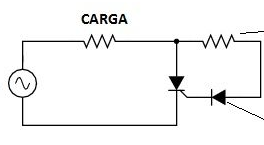
\includegraphics[width=9cm]{SCRenCA-CA.png} 
\caption{SCR en CA-CA}
\end{figure}

En una fuente de corriente alterna es necesario poner una resistencia para que el tiristor no le cause ningun problema y tener un diodo para que la puerta nunca se active en la puerta negativa de la onda.

\begin{figure}[h]
\centering
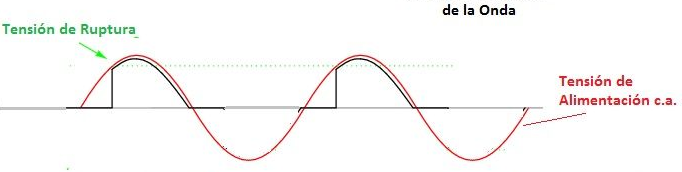
\includegraphics[width=15cm]{RUPTURA.png} 
\caption{Tension en onda}
\end{figure}

Como observamos en la figura anterior nos explica como se ve el trabajo de un tiristor en una onda indicando que en la parte negativa de la onda no hay corriente ya que esta polarizado de manera inversa el tiristor.

\subsection{Operacion de un tiristor SCR por CD}
En el disparo del tiristor por corriente directa en las imagenes anteriores se observa una aplicacion sencilla del tiristor en corriente continua. El tiristor se comporta como un circuito abierto hasta que hasta que se activa una compuerta o switch haciendo llegar poca corriente a travez del interruptor, al proporcionar un pulso al tiristor este se encontrara en estado de conduccion encendiendo la carga o led. En el disparo de corriente continua no necesita ninguna senal adicional para retener la conduccion del tiristor. Una vez activo el tiristor se mantiene conduciendo mientras la corriente del anodo sea mayor que la corriente del mantenimiento. Normalmente la compuerta no tiene control sobre el tiristor una vez que queda conduciendo pero se puede desactivar de la siguiente manera: \begin{enumerate}
\item Abriendo el circuito del anodo
\item Se polariza inversamente el circuito anodo - catodo (El anodo tendra un nivel de tension mayor que el del anodo)
\item Derivando la corriente del anodo, de manera que esta corriente se reduzca y sea menor que la corriente de mantenimiento.
\end{enumerate}

\subsection{Operacion de un tiristor SCR por CA}
La corriente tiene que ser menor que la corriente maxima que puede soportar el tiristor en el anodo y el catodo cuando este entre en conduccion o se active este valor se puede modificar en la hoja de datos del tiristor que se utilice como IMRS. A travez de esta corriente el tiristor se puede calcular la resistencia que garantice que el tiristor se activara (o evitar una tragedia) aplicando la ley de kirchoff en la malla de compuerta para eso es necesario saber la corriente de disparo IGT asi como su tension de disparo. 

\end{document}
